\chapter{Introduction}
\markright{Huijuan Shao \hfill Chapter 1. Introduction \hfill}

\emph{Analytics} has transformed the perception of the world we live in. Big Data is the lingua franca of the twenty first century and data science has become an essential lens through which decision making is seen. The massive amounts of data collected via several active and passive instrumentations positions us truly in \emph{age of information}. Data via web 2.0, social media, internet of things, traffic flow, gene sequencing, etc. in conjunction with advancement of data mining & machine learning to glean actionable insights has influenced the world in designing policy, pricing products, launching political campaigns, and many other applications. The power of \emph{data analytics}, thus, is in its diversity. One such application is in \emph{urban computing}. It has been projected that by the year 2030, cities will grow by 590,000 square miles and add an additional 1.47 billion people, so that 6 out of every 10 people will live in a city. Key issues concerning urban populations, such as public health, sustainable use of limited energy resources, emergency preparedness, and societal stability will rise to the forefront. A data scientist role has become critical in being able to learn, process, analyze, and deliver insights that can help realize the promises of this \emph{unprecedented urbanization}. Towards that end, one of the critical components which has long been a topic of research interest but has found resurgence in this era of urbanization is tackling problems of energy consumption. The relevance of the problem is two-fold. The immediate impact that urbanization has presented us with logistical problems and the larger impact is one that energy has on the environment. Climate-change is a huge problem that will have an impact on humanity as we know it. It is a problem that needs a several pronged attack to find a solution and finding solutions to problems in energy consumption, reducing the carbon footprint, would be a big step forward. 

One of the essential resources in today's world is power and electricity. Electricity usage permeates all aspects of modern society.
Its most conspicuous
uses include urban contexts such as
lighting, air conditioning, refrigeration, heating, and, powering
appliances and gadgets but its penetration is pervasive across rural
and industrial sectors.
In 2014, the residential and commercial sector
comprised nearly 40\% of all the electricity generated in the U.S. \cite{book2014us}.
Furthermore, our dependence on electricity will continue to grow
as emphasis shifts away from fossil fuel based vehicles to electric
vehicles.

While people generally agree on the importance of conservation and
usage curtailment, they are often at difficulties to quantify 
{\em where, when} and {\em how much} electricity is consumed.
Typically, residences and businesses receive
monthly electricity bills indicating aggregate usage, with no information on
the breakdown of consumption by appliances/devices, time of day, or day of
week (this is an area in great flux, however). Research has 
shown that simply making such feedback available to users
can reduce consumption by up to 50\%, although typical saving 
are in the 9\% to 20\% range \cite{book2014us}.%\cite{energydatabook2011}.

One obvious approach to determining the breakdown of consumption is to install
power meters in every circuit (and sub-circuit)
to capture consumption of individual devices in homes and
offices. Such installation is costly and intrusive, making 
this option unviable in practice. 
An alternate
solution, called energy disaggregation or non-intrusive load monitoring
(NILM),
first proposed by Hart~\cite{hart1992}, is to use analytics to 
{\em infer} the breakdown of consumption from an aggregate 
power measurement of a
site. This drastically reduces the number of meters required per 
home/installation, typically to just one. Furthermore, depending on the analytics desired, it is possible to
use the measurements already being recorded by a utility meter for
disaggregation, especially in cases where utility companies have deployed
smart meters.
Energy disaggregation is hence today a booming area offering both
challenging problems for data analytics and having practical relevance in a
number of areas including sensor networks and building analytics.

Another approach to save energy in homes is to 
efficiently use electricity devices.  
In residential buildings, 
the biggest consumer of electricity is usually the HVAC 
(heating, ventilation, and cooling) system, which generally accounts for ~54\% 
of the buildings electricity consumption~\cite{book2014us}. 
How to automatically start up and shut down the HVAC unit 
is thus a key problem. 
One solution is to predict the occupancy at home 
is to begin by analyzing the activities of daily life 
inside the building. 
Based on the occupancy information, 
an automatic control system can be installed
to operate the HVAC. 

In this work we make efforts to resolve these smart building research with 
temporal mining approaches.
\begin{enumerate}
	\item We present a survey on energy disaggregation from the perspective of data mining features and supervised, semi-supervised and unsupervised algorithms. 
	\item The temporal mining approach motif mining works effectively for energy disaggregation. 
	\item We utilize multivariate piecewise motif mining algorithm for both energy disaggregation and water disaggregation. 
	\item The episode-based model Episode Generating HMM (EGH) and a mixture of EGHs performs well for event prediction in occupancy prediction. 
	%\item It can be used for supervised learning disaggregation and semi-supervised learning approach, even for un-supervised learning approach. 
\end{enumerate}
\section{State of the art}
We open the thesis by defining energy disaggregation formally. Briefly, the goal of energy disaggregation is to effectively break down appliance level power consumption. 



%A related problem pertains to
%non-invasive indoor activities tracking.
%The goal here is to predict the locations of people inside a building
%without the use of invasive cameras.

%\section{Timeline}
%The first proposed
%research problem
%on energy disaggregation has been completed although 
%the work will be extended to time-based motif mining and 
%a new probabilistic models.
%The second task of activity of daily life patterns is underway. 
%The third subject on non-invasive indoor activities tracking 
%will start in this Oct.. 
%A timeline of activities is shown in Figure~\ref{fig_PhDtimeline}. 

%\begin{figure}[!hbtp]
%\centering
%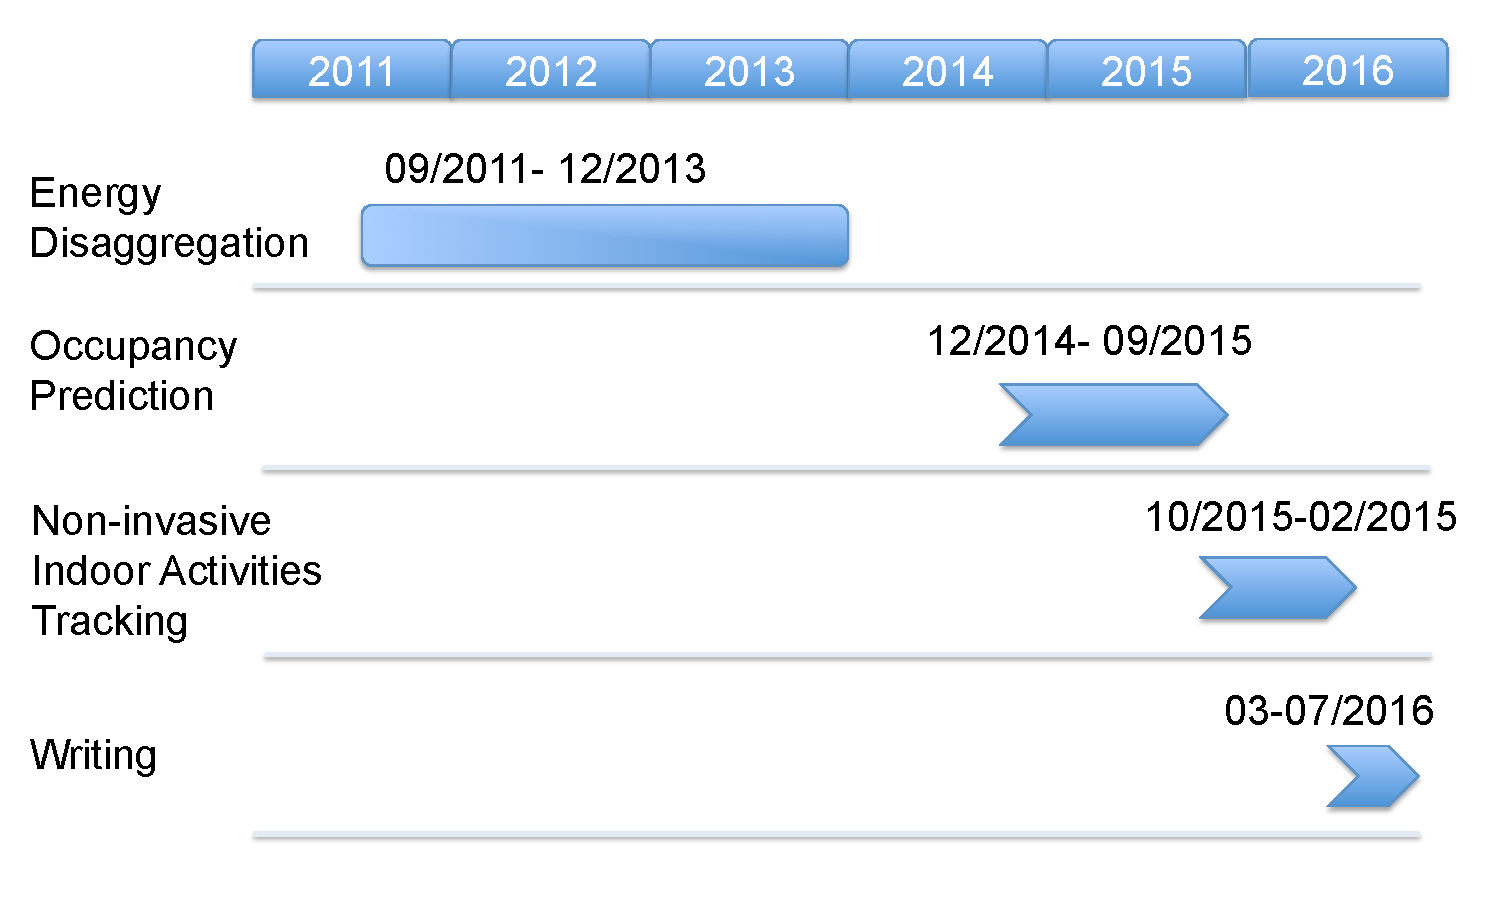
\includegraphics[width=0.8\textwidth]{fig/PhDTimeline.pdf}
%\caption{Timeline.\label{fig_PhDtimeline}}
%x\end{figure}
